\begin{frame}{Synchrotron techniques}

\begin{table}[]
    \centering
    \small
    \begin{tabular}{l|l|l|l}
        Technique & Sample & Sensitivity & Information \\
        \hline
        \hline
        \textcolor{Important}{Surface X-ray} & Pt monocrystals & Surface & Roughness, relaxation\\
        \textcolor{Important}{Diffraction (SXRD)} & (111), (100) & structure & and crystallographic phases \\
        \hline
        \pause
        \onslide<2->{\textcolor{Blue}{X-ray Photoelectron}}  & \onslide<2->{Pt monocrystals} & \onslide<2->{Surface} & \onslide<2->{Species presence,} \\
        \onslide<2->{\textcolor{Blue}{Spectroscopy (XPS)}} & \onslide<2->{(111), (100)} & \onslide<2->{species} & \onslide<2->{quantity, oxidation state} \\
        \hline
        % \pause
        \onslide<3->{\textcolor{Important}{Bragg Coherent}} & \onslide<3->{Pt nanoparticles} & \onslide<3->{Bragg electronic} & \onslide<3->{Shape, 3D strain}  \\
        \onslide<3->{\textcolor{Important}{Diffraction Imaging}} & \onslide<3->{(111), (110), (100), ...} & \onslide<3->{density} & \onslide<3->{and displacement arrays} \\
        \onslide<3->{\textcolor{Important}{(BCDI)}} & \onslide<3->{} & \onslide<3->{} & \onslide<3->{}\\
    \end{tabular}
    \caption{Near-ambient pressure (NAP) X-ray techniques carried out at \textcolor{Important}{SixS} (SOLEIL) or \textcolor{Blue}{B-07} (Diamond) synchrotrons for the present study.}
    \label{tab:techniques}
\end{table}

\vspace{-0.5cm}

% \begin{figure}
% \centering
    % \onslide<2->{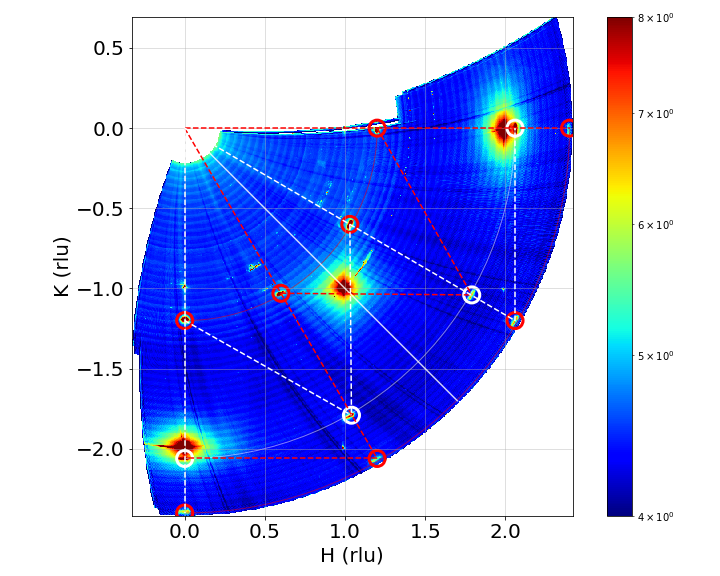
\includegraphics[width=0.45\textwidth]{Figures/sxrd_data/maps/Map_hkl_surf_or_2227-2283.png}}
    %%%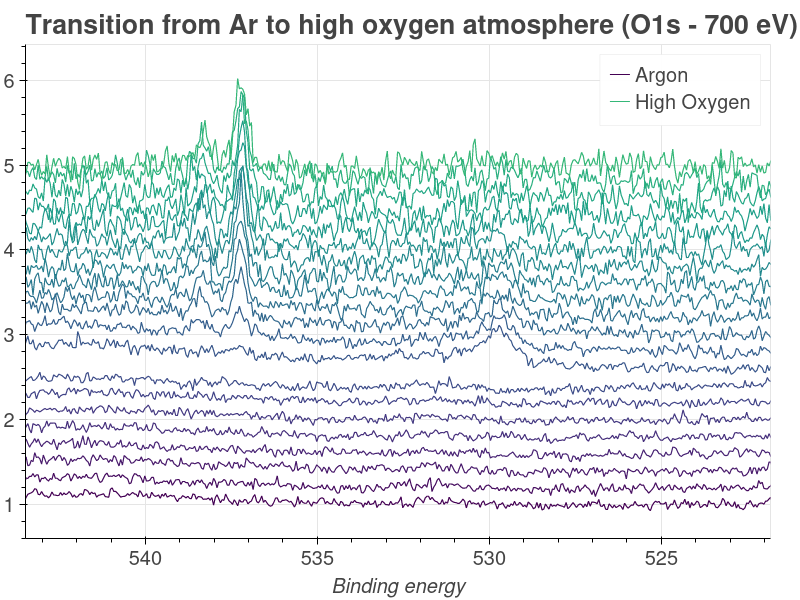
\includegraphics[width=0.32\textwidth]{Figures/xps_data/transition_xps.png}
    %%% 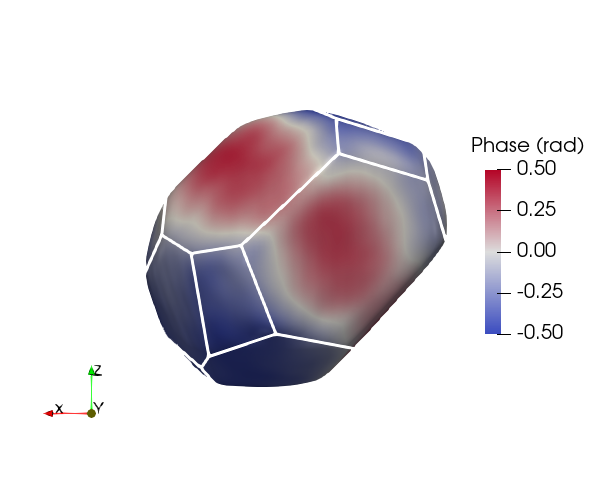
\includegraphics[width=0.42\textwidth]{Figures/gwaihir/facets_D6.png}
    % \onslide<2->{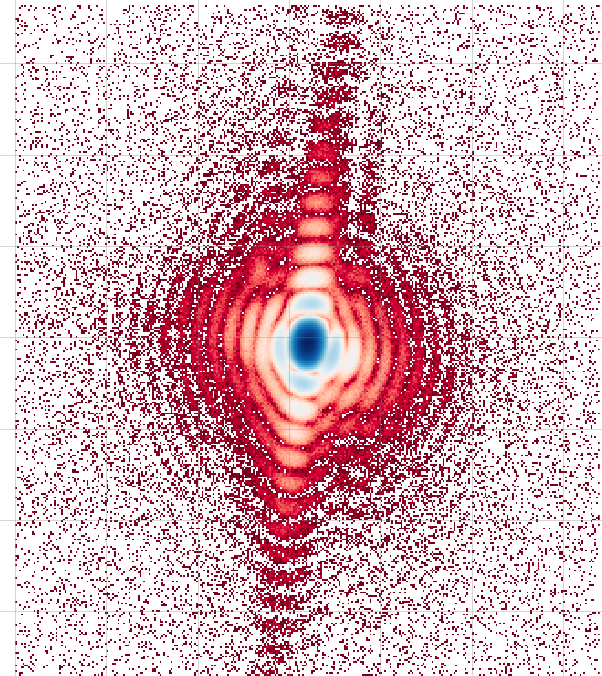
\includegraphics[width=0.35\textwidth]{Figures/gwaihir/dp_pr.png}}
% \end{figure}

\begin{center}
\hspace{-0.5cm}
    {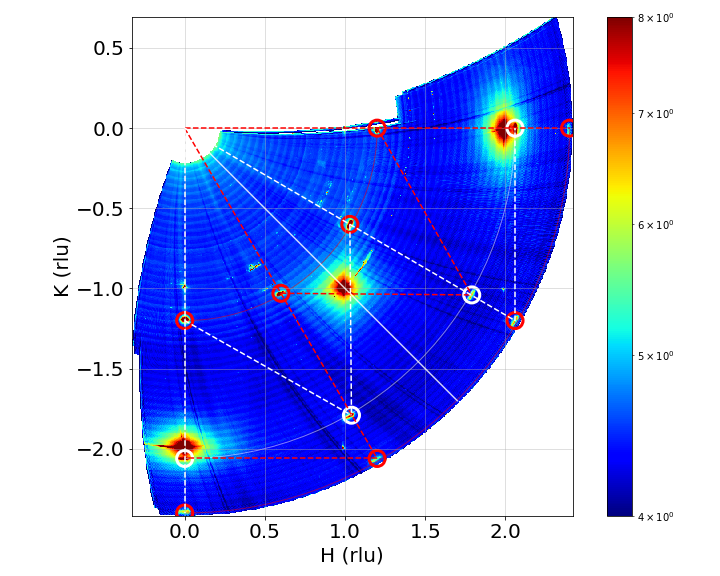
\includegraphics[height=0.45\textheight]{Figures/sxrd_data/maps/Map_hkl_surf_or_2227-2283.png}}
    \onslide<2->{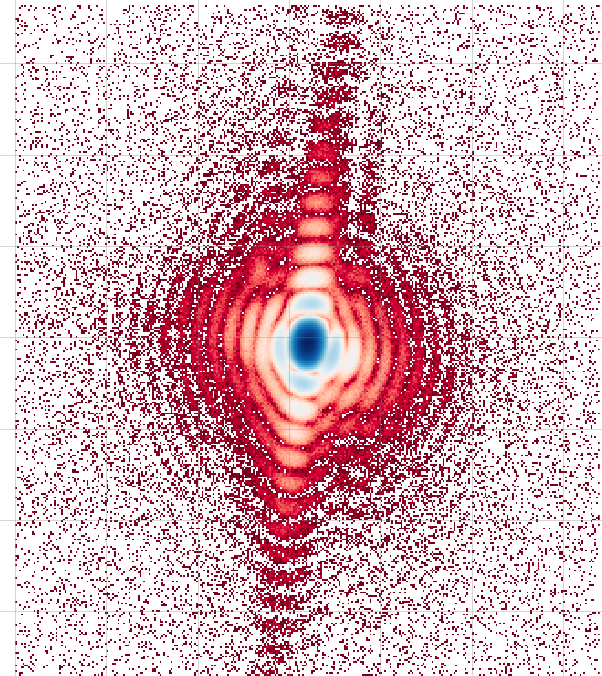
\includegraphics[height=0.35\textheight]{Figures/gwaihir/dp_pr.png}}
    \onslide<3->{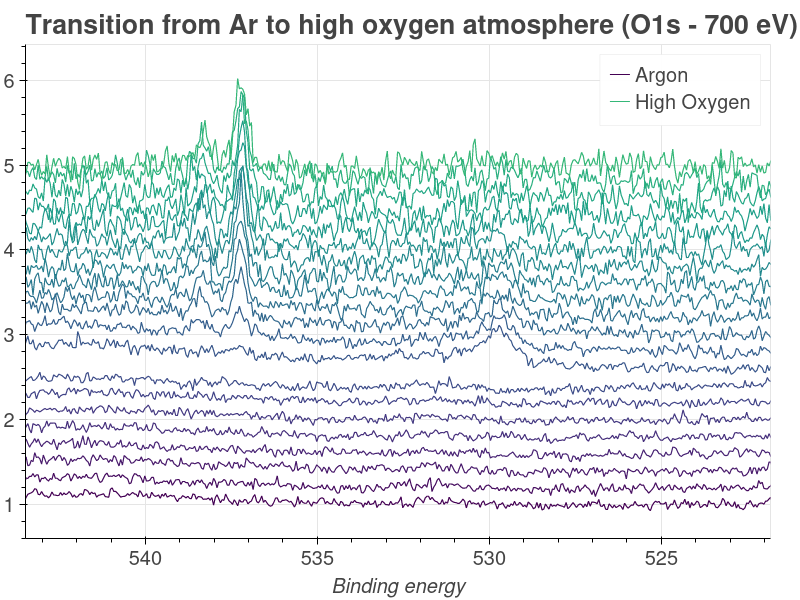
\includegraphics[height=0.32\textheight]{Figures/xps_data/transition_xps.png}}
\end{center}    
    
\end{frame}